\makeatletter
\makeatother
\documentclass[10pt,english]{article}\usepackage{graphicx, color}
%% maxwidth is the original width if it is less than linewidth
%% otherwise use linewidth (to make sure the graphics do not exceed the margin)
\usepackage{alltt}
\usepackage[T1]{fontenc}
\usepackage[latin9]{inputenc}
\usepackage{geometry}
\geometry{left=1.5cm,right=1.5cm,top=2cm,bottom=2cm}
\usepackage{fancyhdr}
\pagestyle{fancy}
\setlength{\parskip}{\smallskipamount}
\setlength{\parindent}{0pt}
\usepackage{amsthm}
\usepackage{amsmath}
\usepackage{subfigure}

\makeatletter

%%%%%%%%%%%%%%%%%%%%%%%%%%%%%% LyX specific LaTeX commands.
\providecommand{\LyX}{L\kern-.1667em\lower.25em\hbox{Y}\kern-.125emX\@}

%%%%%%%%%%%%%%%%%%%%%%%%%%%%%% Textclass specific LaTeX commands.
\numberwithin{equation}{section}
\numberwithin{figure}{section}

\@ifundefined{date}{}{\date{}}
%%%%%%%%%%%%%%%%%%%%%%%%%%%%%% User specified LaTeX commands.
\pagestyle{empty} 

\makeatother

\usepackage{babel}
\begin{document}

\title{Week4 Report}


\author{Xiaohui Li, Luhuan Wu}

\maketitle


In this week, we further study the ranking node effect on short average path. We focus on the power index $\alpha$, power ratio d and expected degree E this time. In the first step, we check the connectivity of graph and especially the giant component and find the more disconnected graph than expected. Then we conduct the correlation pretest with varying d and mean. Finally we study the effect on average short path in small graph. 

\section{Connevtivity}
We have found that there exists giant component after expected degree 1, but the graph tends to be connected in a much smaller mean level.
\begin{figure}[htbp]
\centering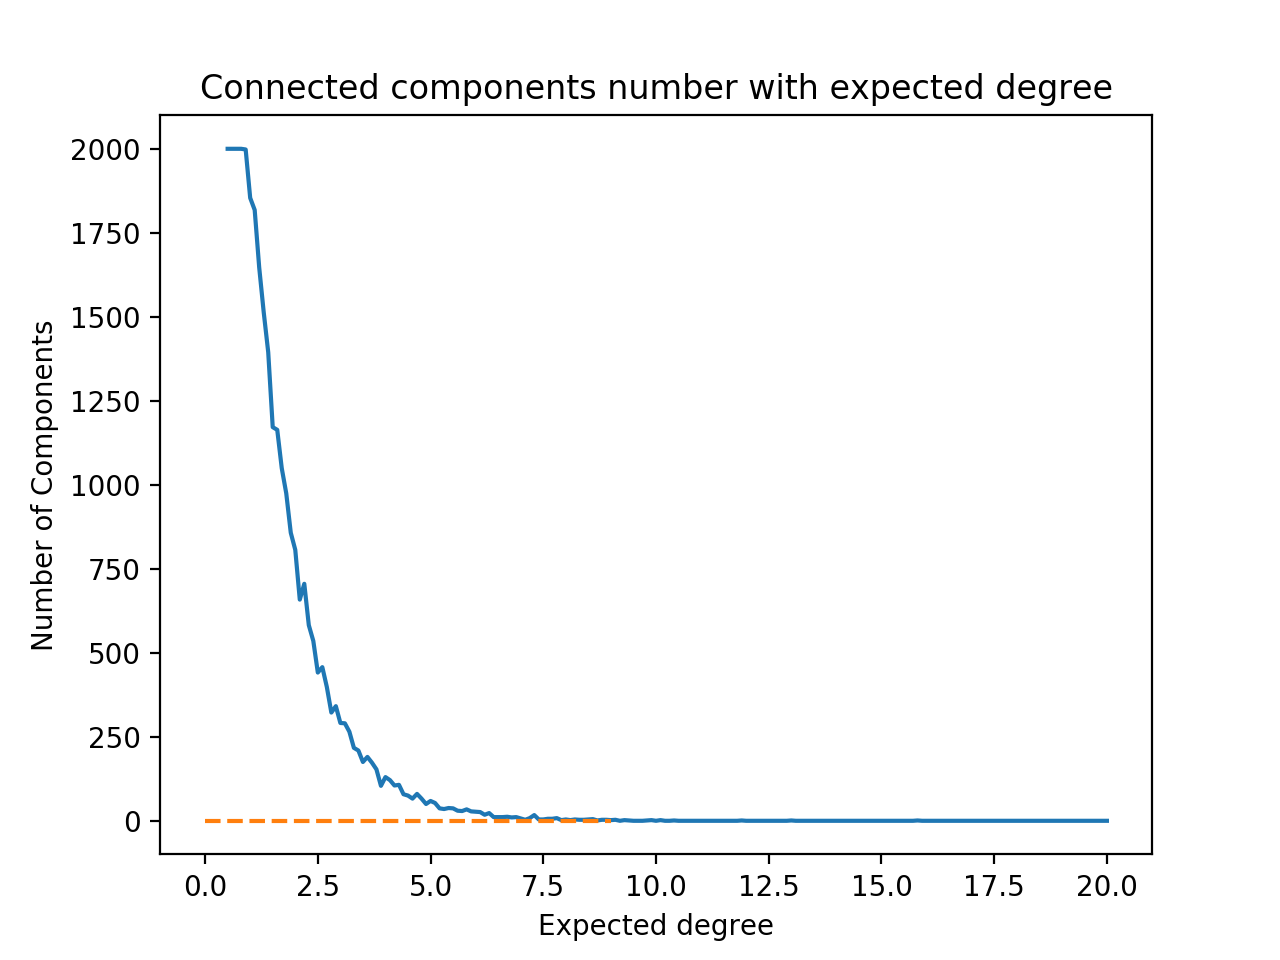
\includegraphics[width=8cm,height= 6cm]{CompoNum}
\caption{Giant components number}
\end{figure}

\begin{figure}[htbp]
\centering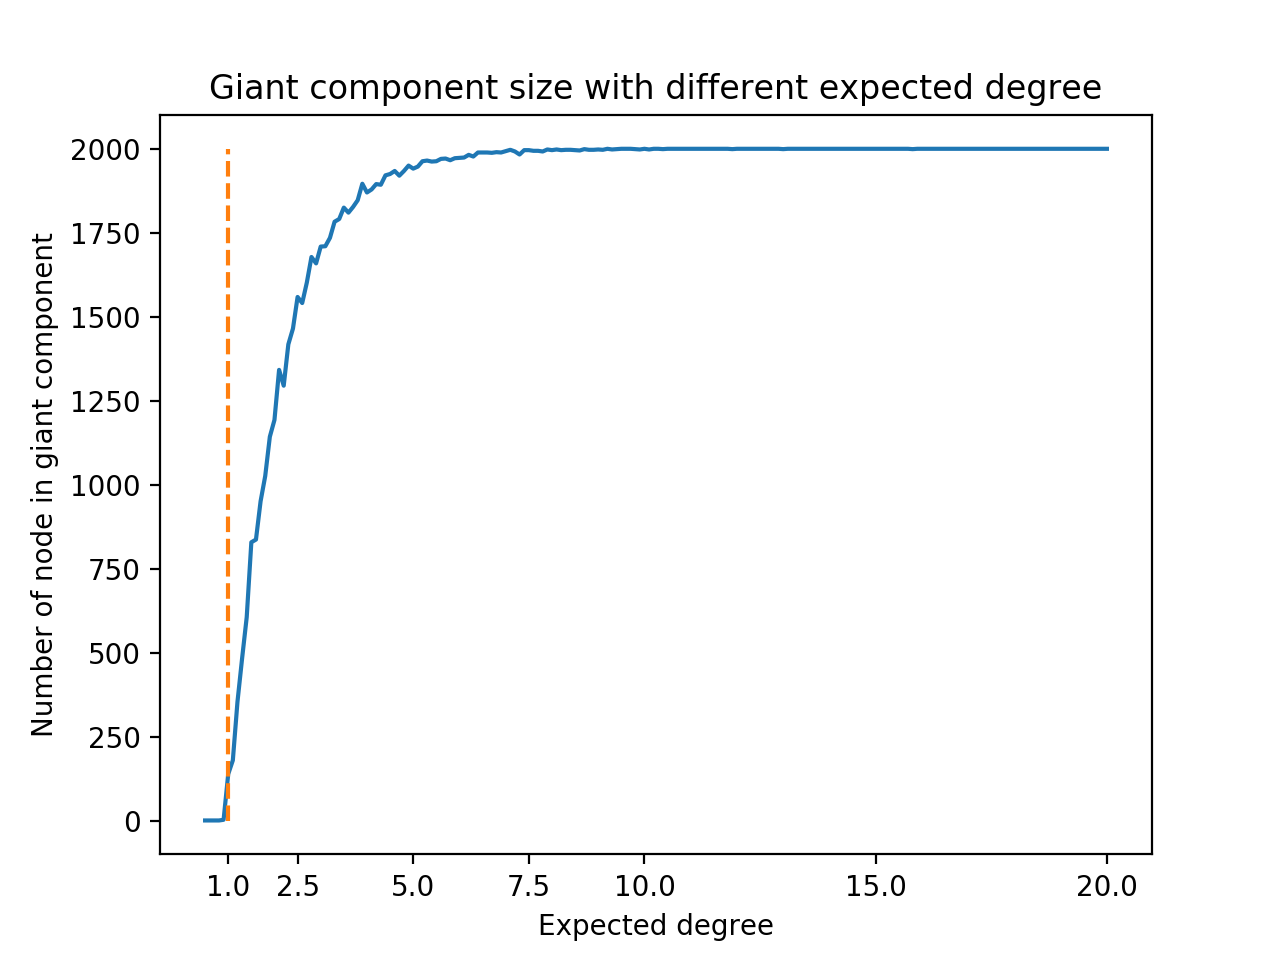
\includegraphics[width=8cm,height=6cm]{GiantCompo}
\caption{Giant component size}
\end{figure}
\quad\\
\quad\\

\section{Correlation}
We make a pretest to see the theoretical correlation relationship with varying d and expected degree E.\\
\begin{figure}[htbp]
\centering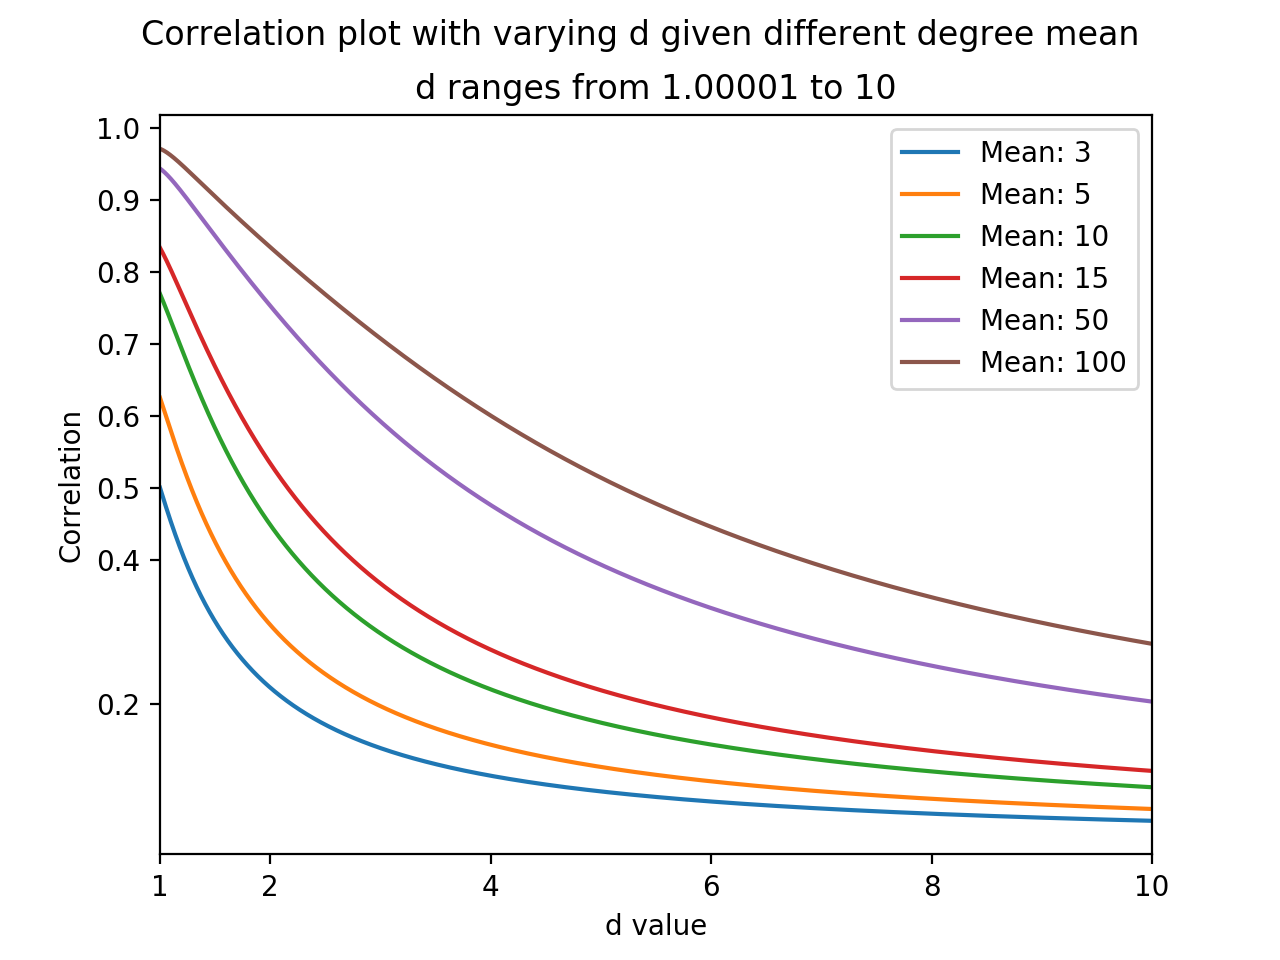
\includegraphics[width=10cm, height=8cm]{correlation}
\caption{Correlation with d given different expected mean}
\end{figure}
\quad\\


\quad\\
\quad\\
\quad\\
\quad\\
\quad\\
\section{Average short path}
For this part, we study the node effect upon average short path, both marginally and individually.\\
\subsection{General graph}
We first test the general graph where in-degree and out-degree are correlated. \\
\quad\\
\subsubsection{Standard graph}
\begin{figure}[htbp]
\centering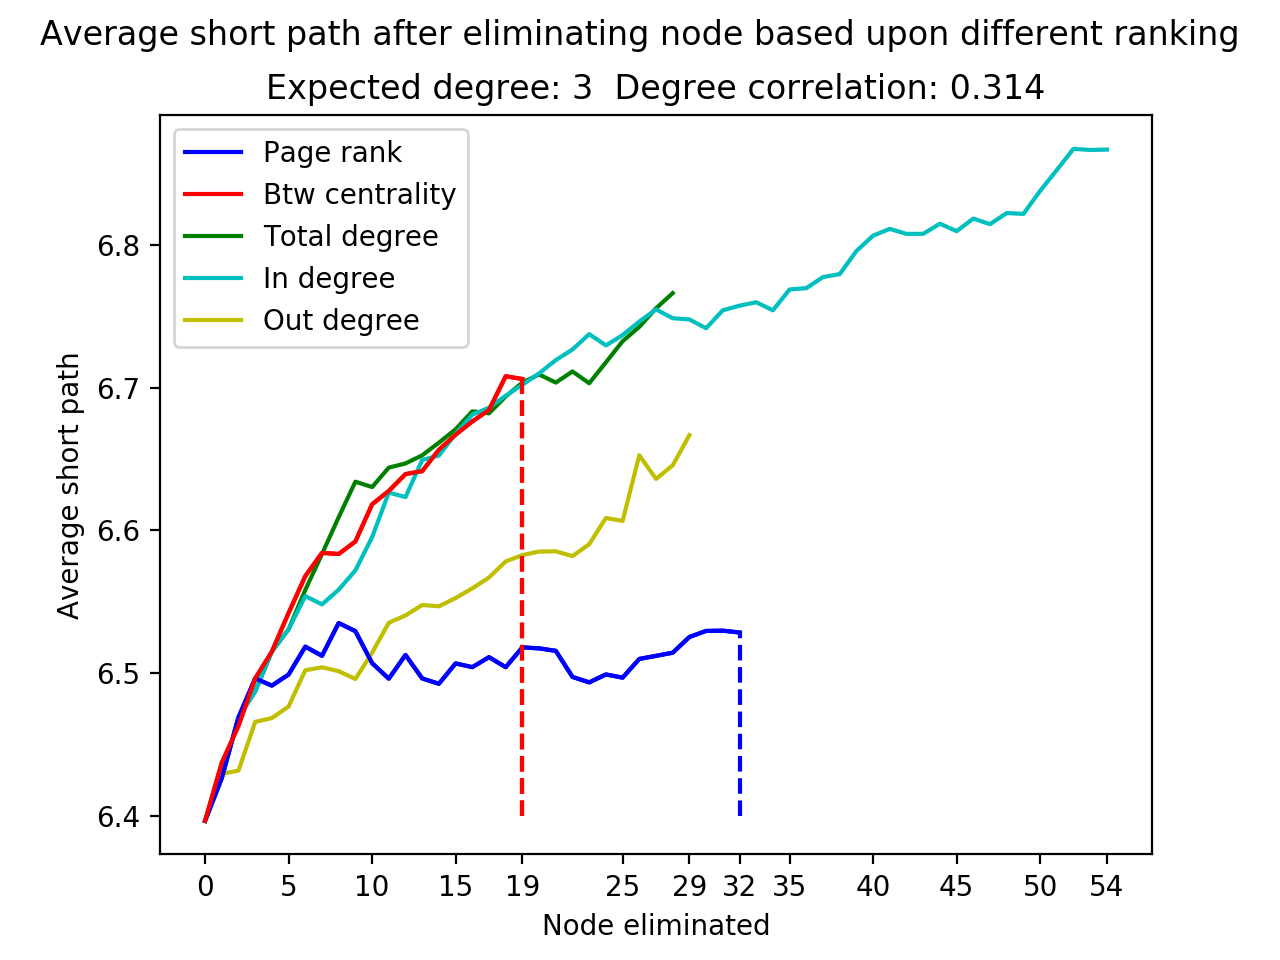
\includegraphics[width=10cm, height=8cm]{avgpath}
\caption{Correlation with d given different expected mean}
\end{figure}
\quad\\

\subsubsection{Comparison}
\begin{figure}[htbp]

\centering\subfigure[High correlation]{
\begin{minipage}{8cm}
\centering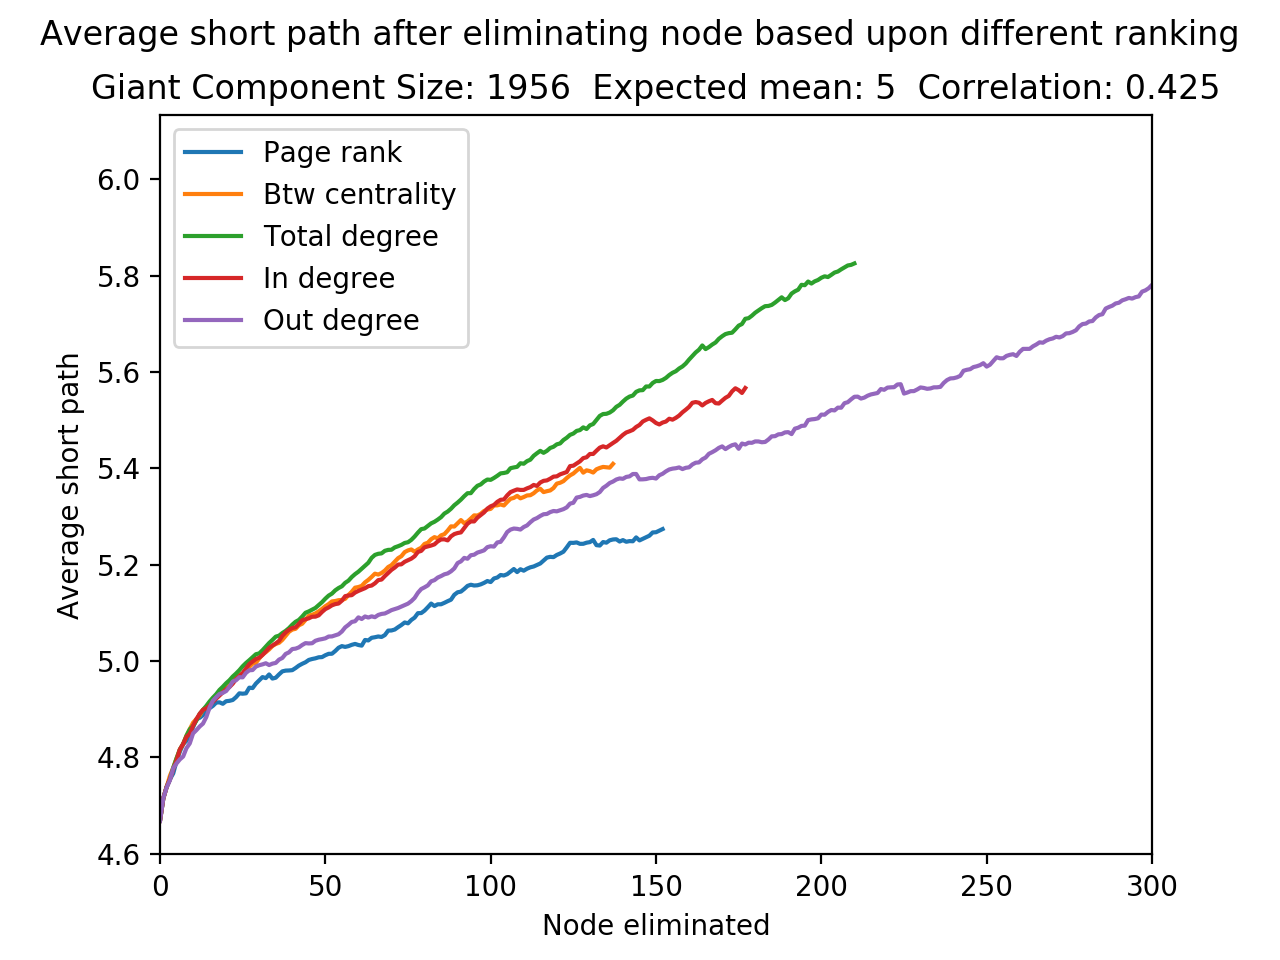
\includegraphics[width=8cm,height=6.2cm]{high}
\end{minipage}
}
\subfigure[Small correlation]{
\begin{minipage}{6cm}
\centering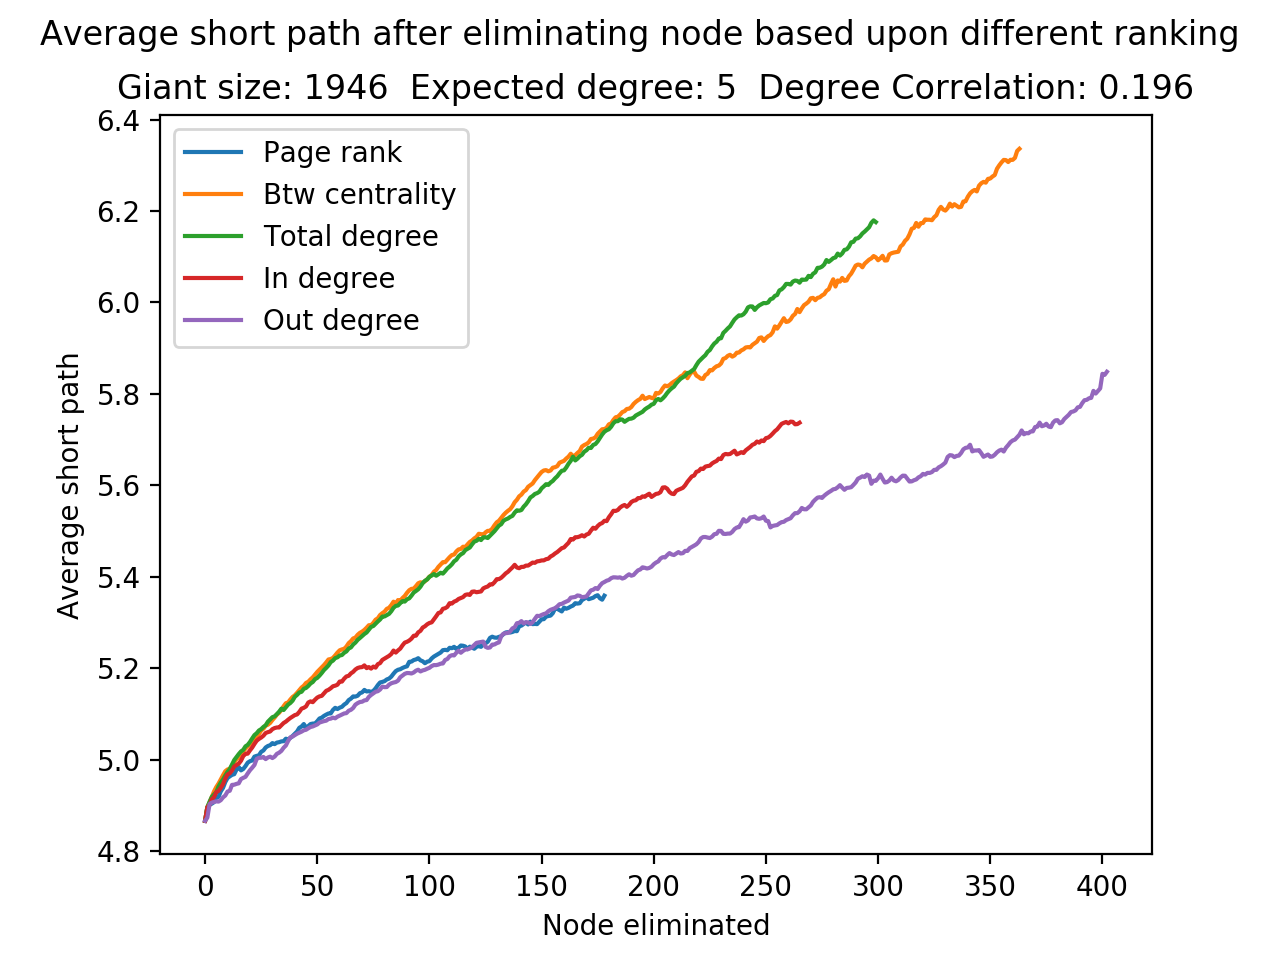
\includegraphics[width=8cm,height=6.2cm]{low}
\end{minipage}
}
\caption{Effect in high and low correlated case}
\end{figure}
\quad\\
\quad\\
\quad\\
\quad\\
\quad\\
\quad\\
\quad\\
\quad\\
\quad\\
\quad\\
\quad\\
\quad\\
\quad\\

\subsection{Extreme sequence}
\subsubsection{Independent degree sequence}

\begin{figure}[htbp]
\centering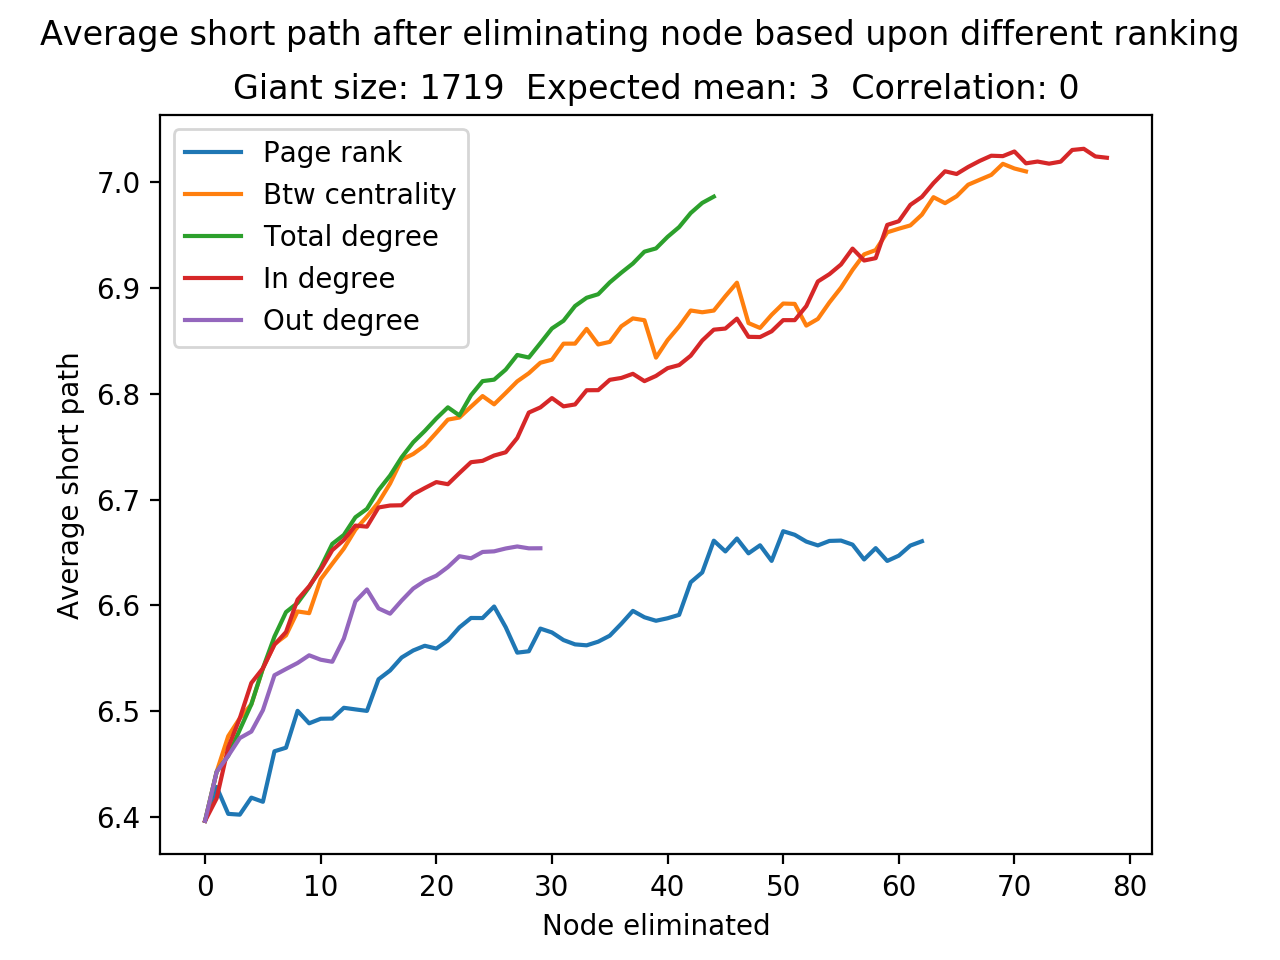
\includegraphics[width=10cm, height=8cm]{avgind}
\caption{Node effect on short average path in independent case}
\end{figure}
\quad\\
\quad\\
\begin{figure}[htbp]

\centering\subfigure[Same power index $\alpha = \beta = 3$]{
\begin{minipage}{8cm}
\centering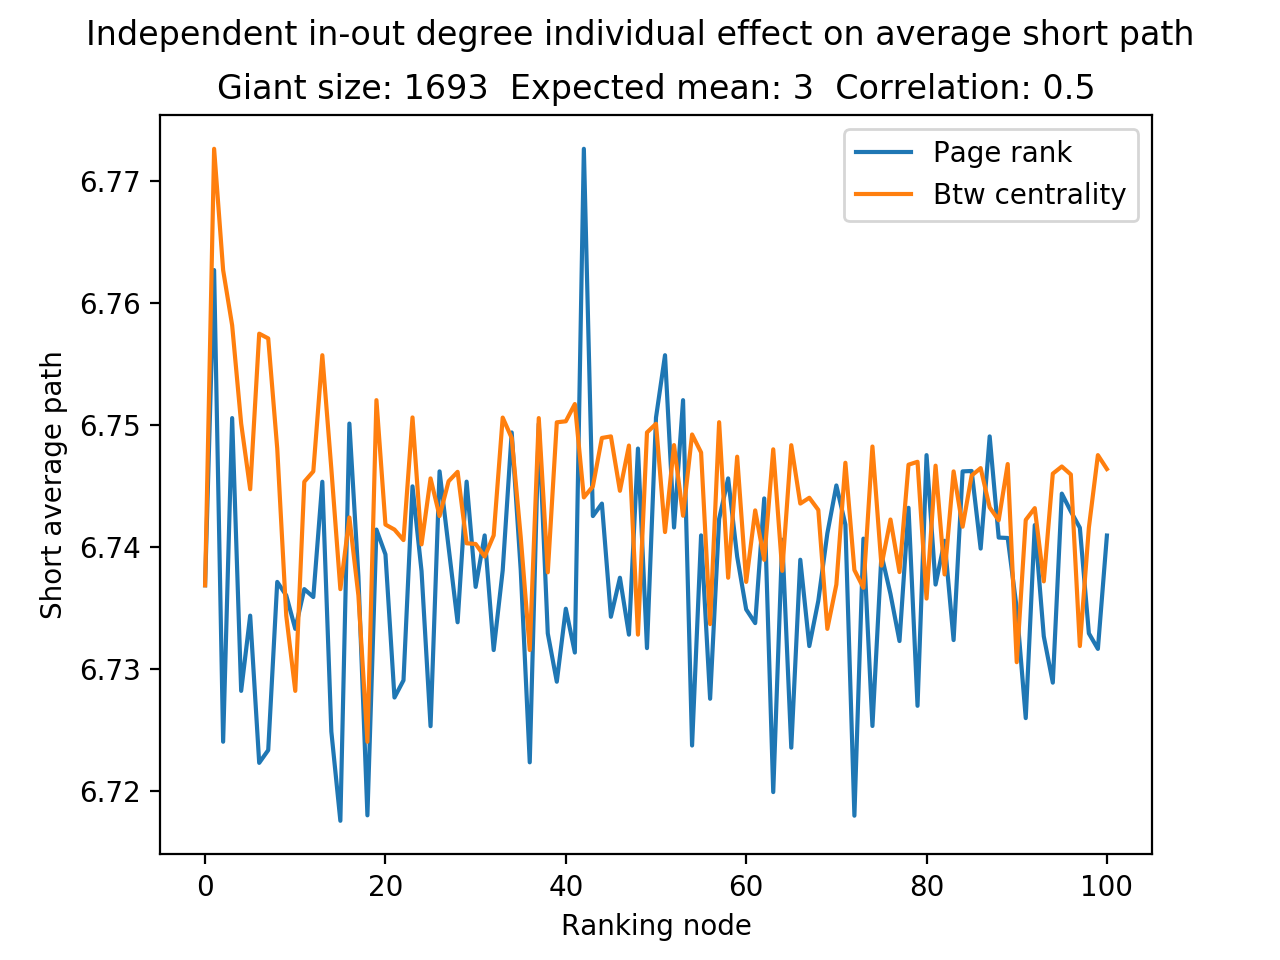
\includegraphics[width=8cm,height=6.2cm]{indepAvg}
\end{minipage}
}
\subfigure[Different power index $\alpha = 3, \beta = 4.5$]{
\begin{minipage}{6cm}
\centering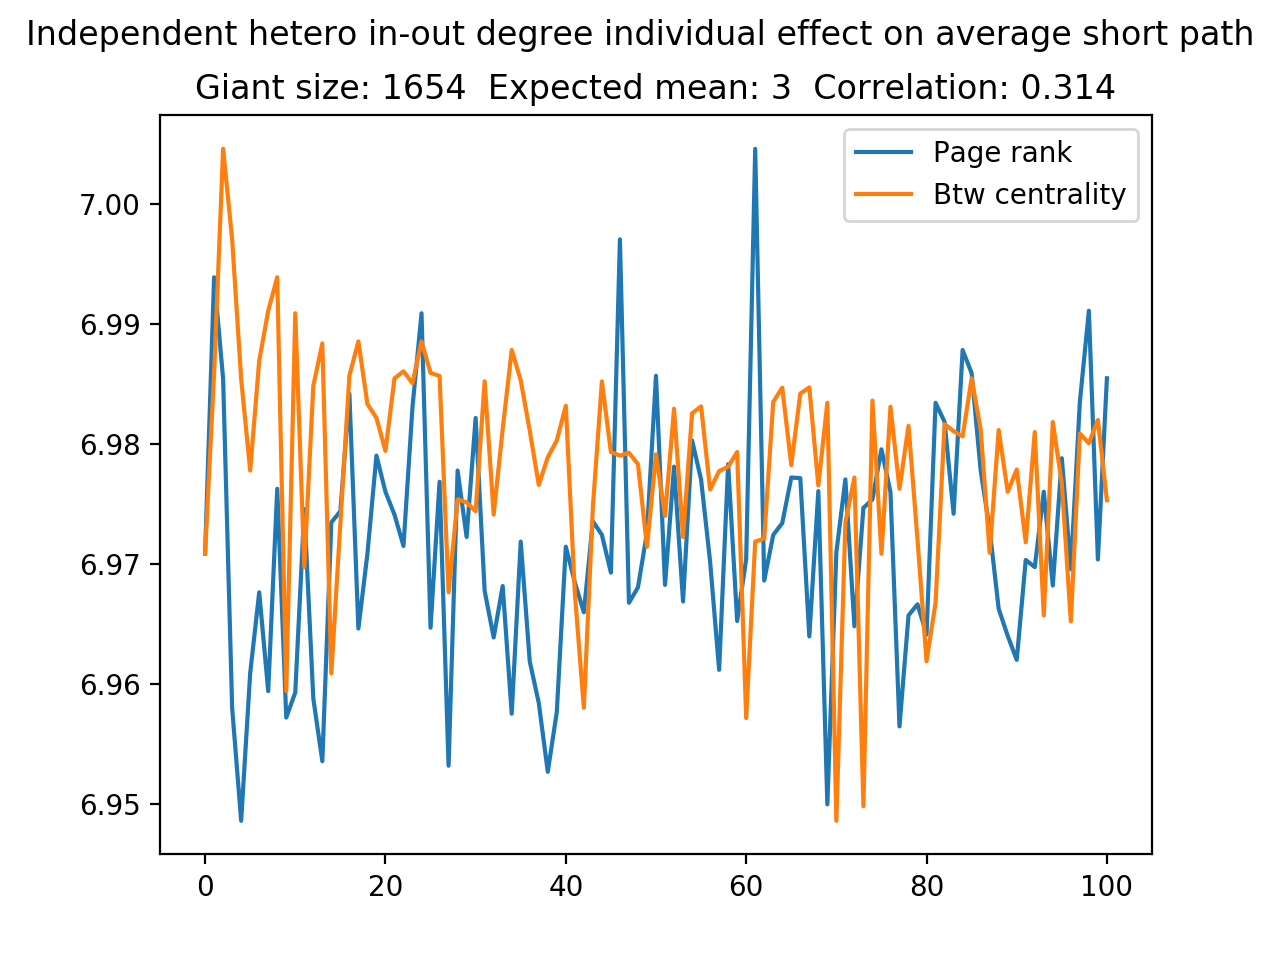
\includegraphics[width=8cm,height=6.2cm]{indepHetAvg}
\end{minipage}
}
\caption{Independent case with same power index and different index ($\alpha$, $\beta$)}
\end{figure}
\quad\\
\quad\\
\quad\\
\quad\\
\quad\\
\quad\\
\subsubsection{Perfectly correlated degree sequence}

\begin{figure}[htbp]
\centering\subfigure[]{
\begin{minipage}{10cm}
\centering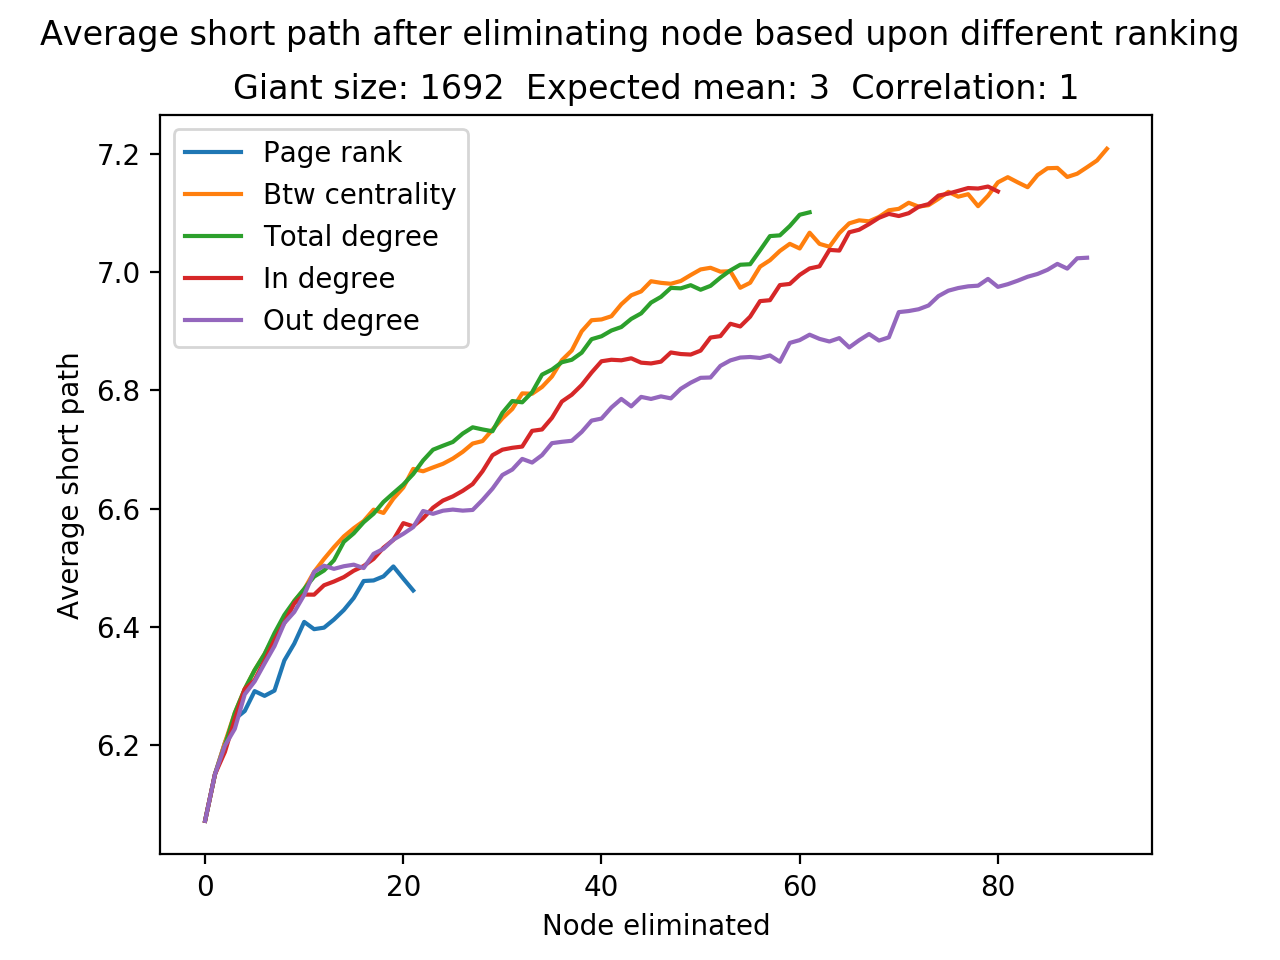
\includegraphics[width=8cm,height=6.2cm]{same}
\end{minipage}
}
\subfigure[]{
\begin{minipage}{6cm}
\centering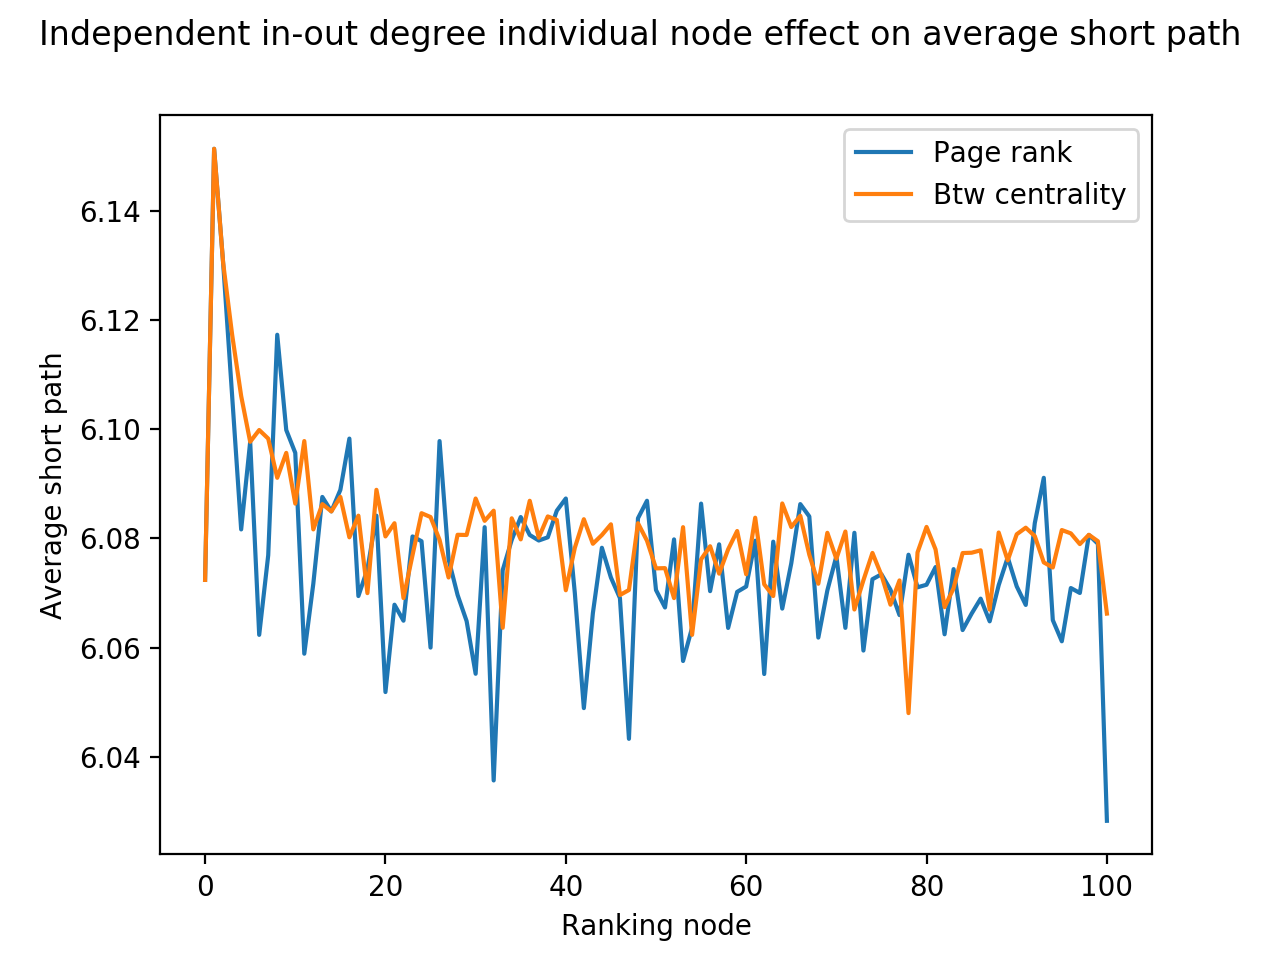
\includegraphics[width=8cm,height=6.2cm]{sameavg}
\end{minipage}
}
\caption{Marginal and individual average effect}
\end{figure}


\end{document}



